% Provenance (never printed): cycle 2 "Explorer les organisations du monde ---
% identifier des paysages" (littoraux, massifs montagneux, campagnes, villes),
% see sources/book1/PROVENANCE.md. Book 1, grade 1, chapter 2.
\chapter{Bentang Alam di Sekitar Kita}\label{ch:g1:landscapes-around-us}

Mia dan kakeknya sudah berjalan jauh mendaki \omterm{def:g1:landscapes-around-us:landform}{bukit} di belakang desa. Di
puncak, mereka duduk di rumput untuk mengatur napas, lalu memandang. Di
bawah mereka, atap-atap merah desa berkerumun di sekitar gereja. Sebuah
\omterm{def:g1:landscapes-around-us:water}{sungai} berkelok-kelok di antara ladang hijau dan kuning, lalu melintas di
bawah jembatan. Ada hutan yang gelap di \omterm{def:g1:landscapes-around-us:landform}{bukit} sebelah. Dan jauh, jauh
sekali, di ujung daratan, tampak segaris tipis warna biru.

``Itu laut,'' kata kakeknya.

Semua yang dapat dilihat Mia dari puncak \omterm{def:g1:landscapes-around-us:landform}{bukit}, yang dekat maupun yang
jauh, adalah sebuah \omterm{def:g1:landscapes-around-us:landscape}{bentang alam}.

\begin{omfigure}
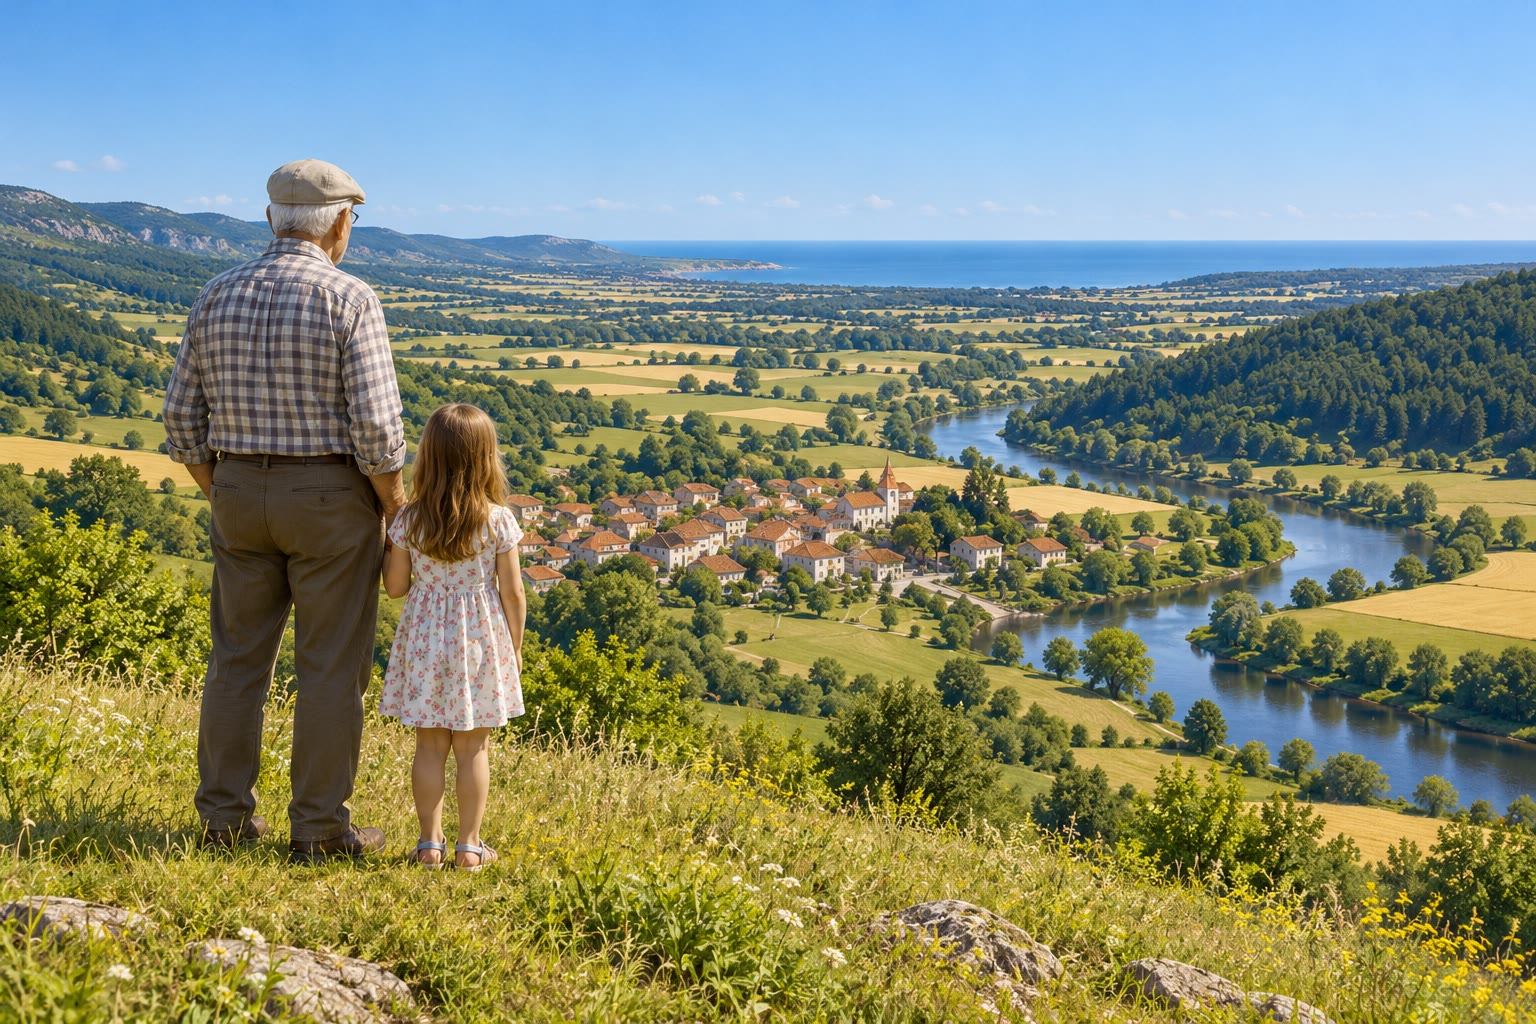
\includegraphics[width=0.72\linewidth]{images/book1/ai/g1-hilltop-view.jpg}

{\small Dari puncak \omterm{def:g1:landscapes-around-us:landform}{bukit} kita melihat seluruh \omterm{def:g1:landscapes-around-us:landscape}{bentang alam}.}
\end{omfigure}

\section{Apa itu bentang alam?}

\begin{definition}[Bentang alam]\label{def:g1:landscapes-around-us:landscape}
Yang disebut \emph{bentang alam}\index{bentang alam} adalah segala sesuatu
di daratan yang dapat kita lihat dalam sekali pandang, dari tempat kita
berdiri sampai ke cakrawala yang jauh: bentuk permukaan tanah, air,
tumbuhan, dan benda-benda yang dibangun manusia.
\end{definition}

\omterm{def:g1:landscapes-around-us:landscape}{Bentang alam} mempunyai bagian yang dekat dan bagian yang jauh. Bagian yang
paling dekat dengan kita ada di bawah dari apa yang kita lihat; bagian itu
tampak besar dan kita melihat rinciannya. Bagian yang jauh ada di atas,
dekat langit; bagian itu tampak kecil dan pucat.

\begin{omfigure}
\begin{tikzpicture}[x=1cm, y=1cm]
  \fill[ocBlue!12] (0,0) rectangle (10,5);
  % background: far hills
  \fill[black!18] (0,3.0) -- (1.5,3.6) -- (3,3.3) -- (5,3.9) -- (7,3.4) -- (8.5,3.8) -- (10,3.3) -- (10,2.9) -- (0,2.9) -- cycle;
  % middle: hills and fields
  \fill[green!35!omLithAlluv] (0,1.6) -- (2,2.4) -- (4,2.1) -- (6,2.7) -- (8,2.2) -- (10,2.5) -- (10,1.5) -- (0,1.5) -- cycle;
  \fill[green!25!omLithAlluv] (0,1.5) rectangle (10,2.95);
  \fill[green!35!omLithAlluv] (0,2.95) -- (2,3.1) -- (4,2.95) -- (6,3.25) -- (8,3.0) -- (10,3.1) -- (10,2.9) -- (0,2.9) -- cycle;
  \foreach \x in {5.6,5.9,6.2} \fill[red!55] (\x,2.25) -- ++(0.12,0.15) -- ++(0.12,-0.15) -- cycle;
  \foreach \x in {5.6,5.9,6.2} \fill[white] (\x+0.03,2.1) rectangle ++(0.18,0.15);
  % foreground
  \fill[green!55!black!60] (0,0) rectangle (10,1.5);
  \foreach \x in {0.8,2.1,8.6} {
    \fill[brown!70!black] (\x-0.06,0.4) rectangle (\x+0.06,0.9);
    \fill[green!45!black] (\x,1.15) circle (0.38);
  }
  % band borders and labels
  \draw[white, line width=1pt, dashed] (0,1.5) -- (10,1.5);
  \draw[white, line width=1pt, dashed] (0,2.95) -- (10,2.95);
  \node[font=\small\bfseries, fill=white, fill opacity=0.8, text opacity=1, inner sep=2pt] at (5,0.6) {latar depan: dekat, besar, banyak rincian};
  \node[font=\small\bfseries, fill=white, fill opacity=0.8, text opacity=1, inner sep=2pt] at (2.7,2.2) {latar tengah};
  \node[font=\small\bfseries, fill=white, fill opacity=0.8, text opacity=1, inner sep=2pt] at (5,4.4) {latar belakang: jauh, kecil, pucat};
\end{tikzpicture}

{\small \omterm{def:g1:landscapes-around-us:landscape}{Bentang alam} yang dilihat dalam tiga lajur: latar depan di bawah,
latar tengah, dan latar belakang yang berbatasan dengan langit.}
\label{fig:g1:landscapes-around-us:bands}
\end{omfigure}

\section{Bentuk-bentuk permukaan tanah}

Permukaan tanah tidak datar di mana-mana. Di beberapa tempat tanah menjulang
tinggi ke langit; di tempat lain tanah turun membentuk cekungan yang
panjang; di tempat lain lagi tanah datar sejauh mata memandang. Kita
memberi nama untuk setiap bentuk.

\begin{definition}[Bentuk muka bumi]\label{def:g1:landscapes-around-us:landform}
Yang disebut \emph{bentuk muka bumi}\index{bentuk muka bumi} adalah bentuk
permukaan daratan.
\begin{itemize}
  \item Sebuah \emph{gunung}\index{gunung} adalah bentuk muka bumi yang sangat
        tinggi dengan lereng yang curam; bagian teratasnya disebut puncak.
        Gunung-gunung yang paling tinggi bersalju di puncaknya, bahkan di
        musim panas.
  \item Sebuah \emph{bukit}\index{bukit} adalah bentuk muka bumi yang lebih
        tinggi daripada daratan di sekitarnya, lebih rendah dan lebih
        bulat daripada gunung.
  \item Sebuah \emph{lembah}\index{lembah} adalah cekungan panjang yang
        rendah di antara bukit-bukit atau gunung-gunung; di dasarnya sering
        ada \omterm{def:g1:landscapes-around-us:water}{sungai}.
  \item Sebuah \emph{dataran}\index{dataran} adalah hamparan tanah yang luas,
        datar, dan rendah.
\end{itemize}
\end{definition}

\begin{omfigure}
\begin{tikzpicture}[x=1cm, y=1cm]
  \fill[ocBlue!10] (0,0) rectangle (12.4,4.6);
  % sea
  \fill[omSea] (10.2,0) rectangle (12.4,0.55);
  % land profile: mountains, valley, hill, plain, coast
  \fill[omLithAlluv!80!green] (0,0) -- (0,2.2) -- (0.9,3.3) -- (1.5,3.0) -- (2.2,4.1)
     -- (2.9,2.6) -- (3.6,1.2) -- (3.9,0.9) -- (4.2,1.2) -- (5.0,2.0) -- (5.7,2.2)
     -- (6.4,1.6) -- (7.0,0.95) -- (8.0,0.8) -- (9.5,0.7) -- (10.2,0.6) -- (10.4,0.55)
     -- (10.4,0) -- cycle;
  \draw[black!60, line width=0.6pt] (0,2.2) -- (0.9,3.3) -- (1.5,3.0) -- (2.2,4.1)
     -- (2.9,2.6) -- (3.6,1.2) -- (3.9,0.9) -- (4.2,1.2) -- (5.0,2.0) -- (5.7,2.2)
     -- (6.4,1.6) -- (7.0,0.95) -- (8.0,0.8) -- (9.5,0.7) -- (10.2,0.6) -- (10.4,0.55);
  % snow caps
  \fill[white, draw=black!50, line width=0.3pt] (1.95,3.72) -- (2.2,4.1) -- (2.45,3.72) -- (2.3,3.78) -- (2.2,3.68) -- (2.08,3.78) -- cycle;
  \fill[white, draw=black!50, line width=0.3pt] (0.72,3.08) -- (0.9,3.3) -- (1.05,3.15) -- (0.9,3.12) -- cycle;
  % river in the valley
  \fill[omSea!90!black] (3.75,0.92) rectangle (4.05,0.98);
  % lake on the plain
  \fill[omSea] (7.6,0.82) ellipse (0.5 and 0.07);
  % village on the plain
  \foreach \x in {8.6,8.85,9.1} {
    \fill[white, draw=black!50, line width=0.3pt] (\x,0.74) rectangle ++(0.18,0.16);
    \fill[red!60] (\x-0.02,0.9) -- ++(0.11,0.12) -- ++(0.11,-0.12) -- cycle;
  }
  % labels
  \node[font=\small, above] at (2.2,4.12) {gunung};
  \node[font=\small, above] at (5.6,2.25) {bukit};
  \node[font=\small] at (3.9,1.85) {lembah};
  \node[font=\small, above] at (8.2,1.5) {dataran};
  \draw[black!60, thin] (8.2,1.5) -- (8.2,0.85);
  \node[font=\small, align=center] at (11.3,1.4) {laut};
  \node[font=\scriptsize, below=2pt, fill=white, fill opacity=0.8, text opacity=1, inner sep=1pt] at (7.6,0.35) {danau};
  \draw[black!60, thin] (7.6,0.45) -- (7.6,0.78);
  \node[font=\scriptsize, below=2pt, fill=white, fill opacity=0.8, text opacity=1, inner sep=1pt] at (10.3,0.35) {pesisir};
  \node[font=\scriptsize, fill=white, fill opacity=0.8, text opacity=1, inner sep=1pt] at (3.9,0.2) {sungai};
  \draw[black!60, thin] (3.9,0.32) -- (3.9,0.88);
\end{tikzpicture}

{\small Bentuk-bentuk permukaan tanah, dari pegunungan sampai ke laut,
dilihat dari samping (tingginya digambar jauh lebih tinggi daripada
sebenarnya).}
\label{fig:g1:landscapes-around-us:profile}
\end{omfigure}

\begin{omfigure}
\begin{minipage}[b]{0.49\linewidth}\centering
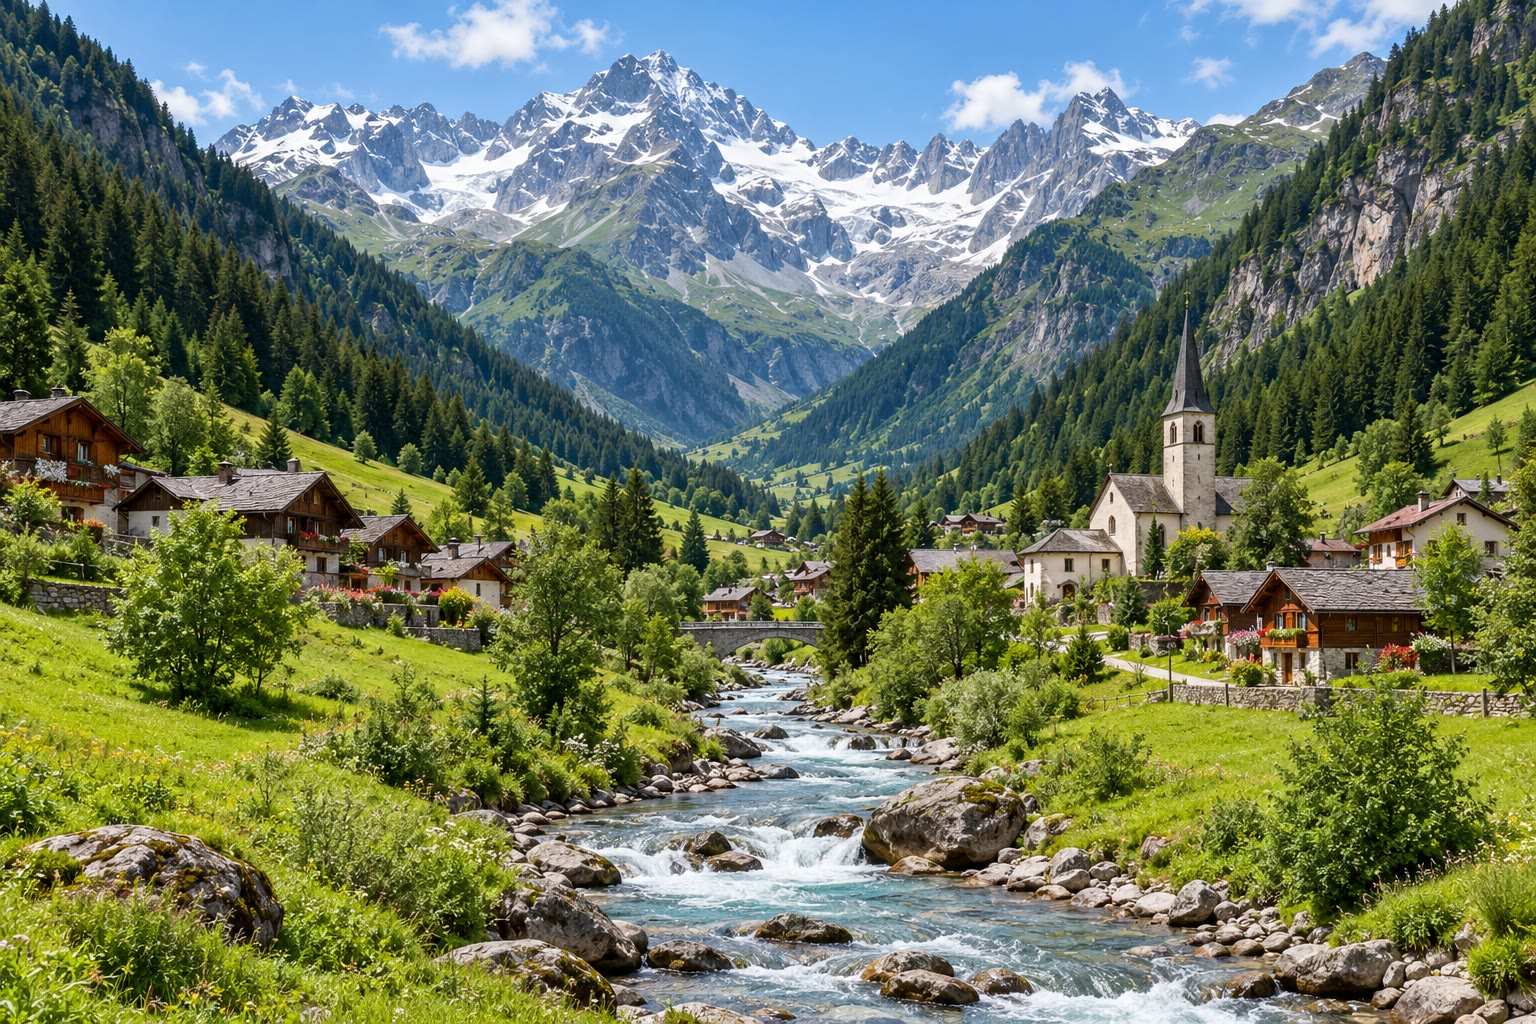
\includegraphics[width=\linewidth]{images/book1/ai/g1-mountain-village.jpg}

{\small \omterm{def:g1:landscapes-around-us:landform}{Gunung-gunung}, dan sebuah desa di \omterm{def:g1:landscapes-around-us:landform}{lembahnya}.}
\end{minipage}\hfill
\begin{minipage}[b]{0.49\linewidth}\centering
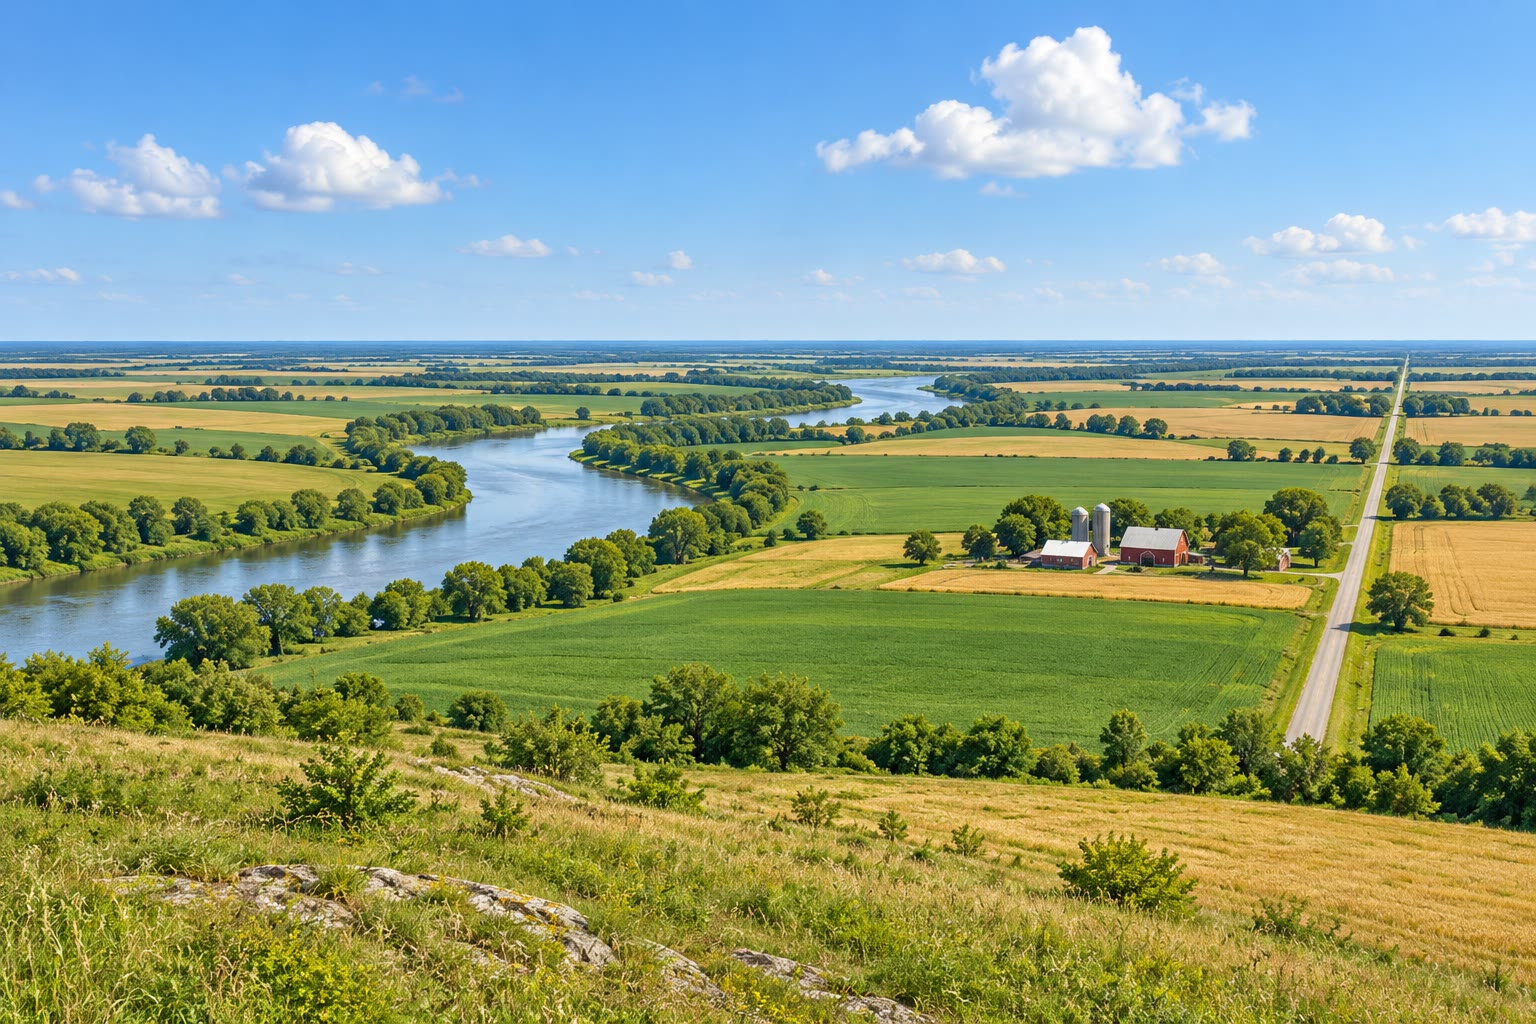
\includegraphics[width=\linewidth]{images/book1/ai/g1-plain-river.jpg}

{\small Sebuah \omterm{def:g1:landscapes-around-us:landform}{dataran}, dengan \omterm{def:g1:landscapes-around-us:water}{sungai} dan ladang.}
\end{minipage}
\end{omfigure}

\begin{example}[Gunung atau bukit?]\label{ex:g1:landscapes-around-us:mountain-hill}
Tidak ada ketinggian pasti saat sebuah \omterm{def:g1:landscapes-around-us:landform}{bukit} menjadi \omterm{def:g1:landscapes-around-us:landform}{gunung}. Kita melihat
bentuknya: \omterm{def:g1:landscapes-around-us:landform}{gunung} itu tinggi dan curam, sering berbatu, kadang-kadang
bersalju di puncaknya; \omterm{def:g1:landscapes-around-us:landform}{bukit} lebih rendah dan lebih bulat, sering ditutupi
rumput, ladang, atau hutan kecil, dan kita bisa berjalan ke puncaknya
dalam waktu singkat.
\end{example}

\section{Air dalam bentang alam}

Air adalah bagian dari kebanyakan \omterm{def:g1:landscapes-around-us:landscape}{bentang alam}. Air mengalir turun dari
\omterm{def:g1:landscapes-around-us:landform}{bukit} dan \omterm{def:g1:landscapes-around-us:landform}{gunung}, berkumpul di cekungan, lalu sampai ke laut.

\begin{definition}[Air dalam bentang alam]\label{def:g1:landscapes-around-us:water}
Yang disebut \emph{sungai}\index{sungai} adalah air yang terus-menerus
mengalir dalam alur yang panjang, dari tanah yang lebih tinggi turun ke
danau atau ke laut. Yang disebut \emph{danau}\index{danau} adalah genangan
air yang besar yang dikelilingi daratan. Yang disebut
\emph{pesisir}\index{pesisir} adalah tempat daratan bertemu dengan laut.
\end{definition}

\begin{omfigure}
\begin{minipage}[b]{0.49\linewidth}\centering
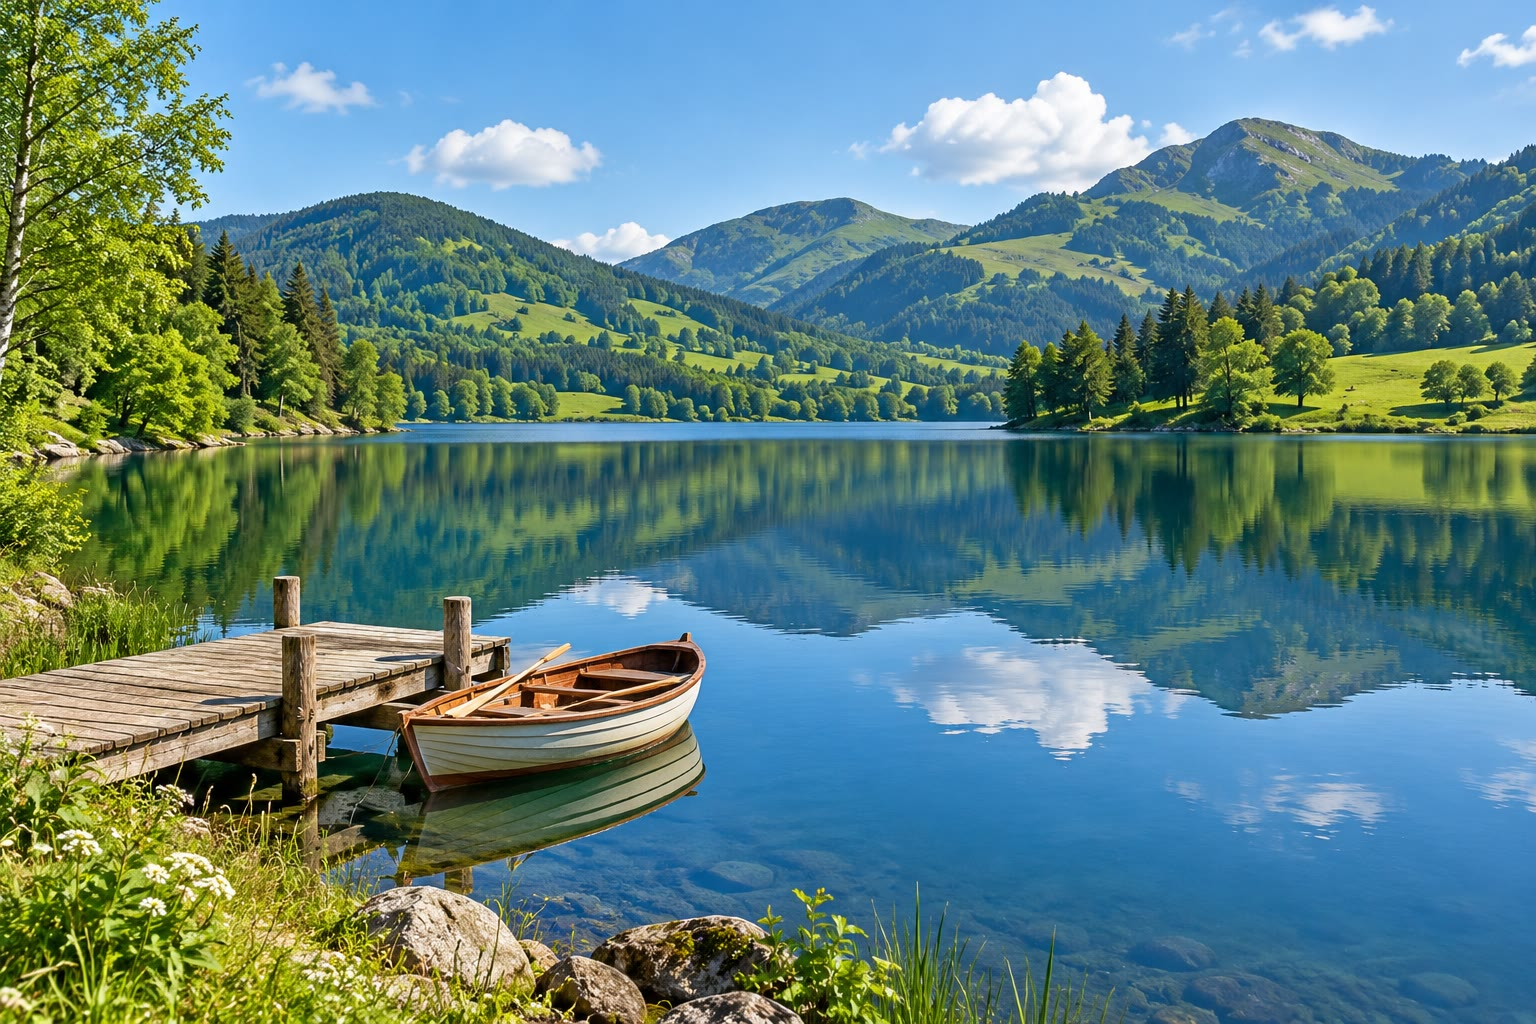
\includegraphics[width=\linewidth]{images/book1/ai/g1-lake-hills.jpg}

{\small Sebuah \omterm{def:g1:landscapes-around-us:water}{danau} di antara \omterm{def:g1:landscapes-around-us:landform}{bukit-bukit}.}
\end{minipage}\hfill
\begin{minipage}[b]{0.49\linewidth}\centering
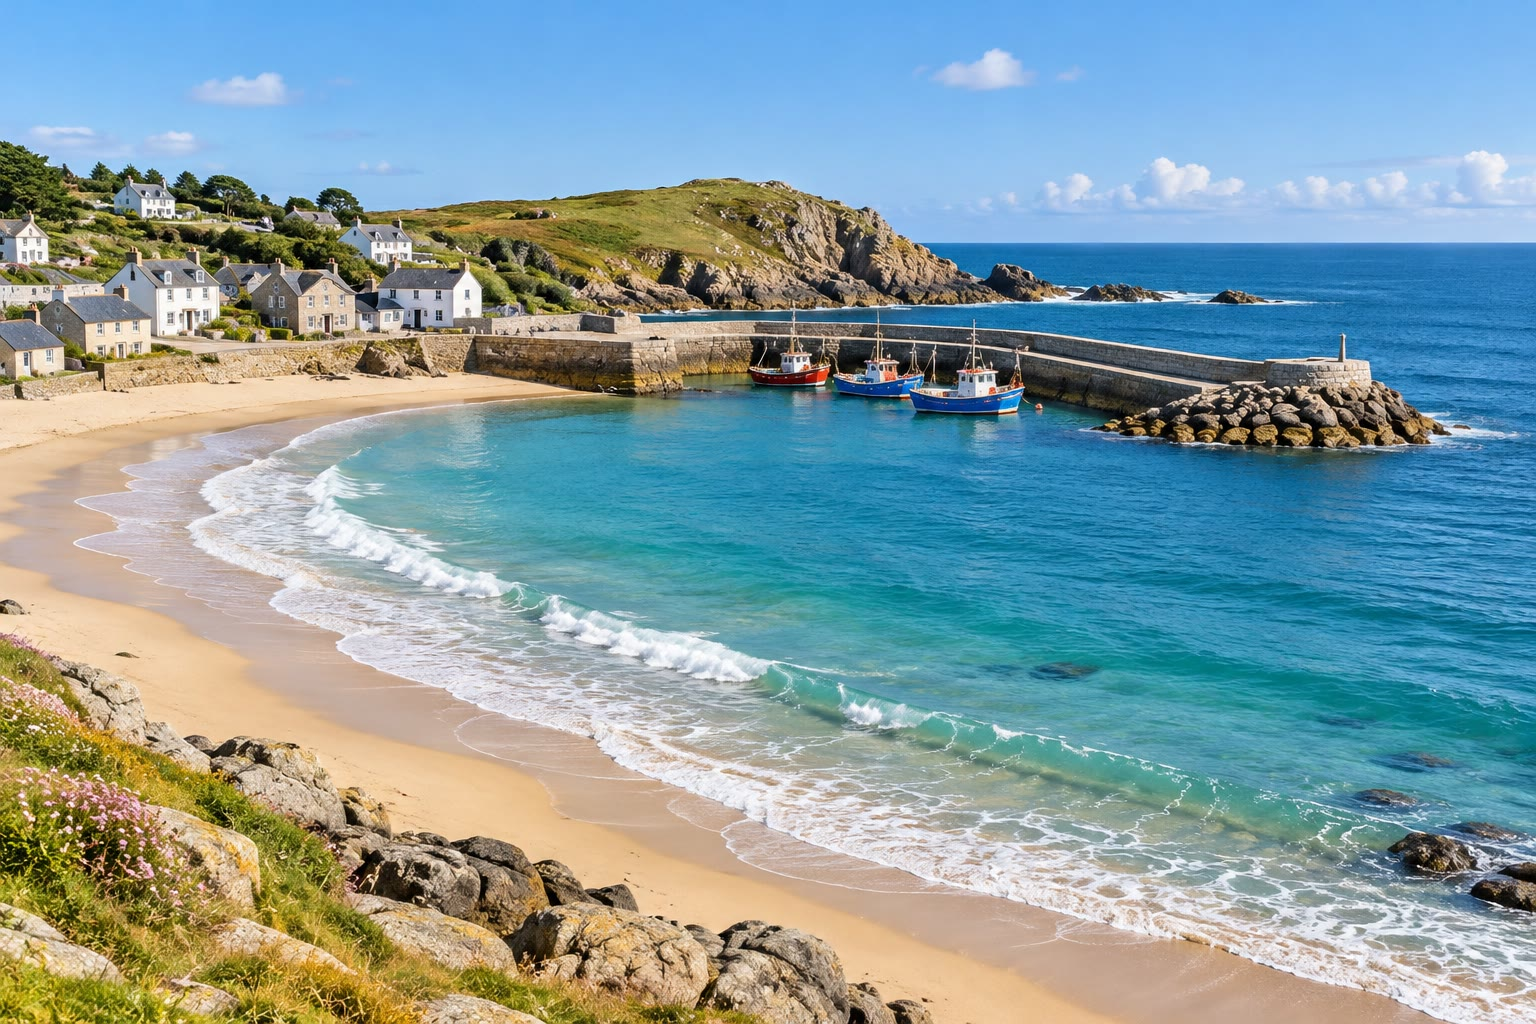
\includegraphics[width=\linewidth]{images/book1/ai/g1-coast-harbour.jpg}

{\small Sebuah \omterm{def:g1:landscapes-around-us:water}{pesisir}: pantai berpasir, batu-batu, dan pelabuhan.}
\end{minipage}
\end{omfigure}

\begin{remark}[Air selalu mengalir ke bawah]\label{rem:g1:landscapes-around-us:downhill}
\omterm{def:g1:landscapes-around-us:water}{Sungai} selalu mengalir dari tanah yang lebih tinggi ke tanah yang lebih
rendah. Itulah sebabnya \omterm{def:g1:landscapes-around-us:water}{sungai} mengalir di dasar \omterm{def:g1:landscapes-around-us:landform}{lembah}, dan mengapa
akhirnya \omterm{def:g1:landscapes-around-us:water}{sungai} sampai ke \omterm{def:g1:landscapes-around-us:water}{danau} atau ke laut, yang lebih rendah daripada
daratan di sekitarnya.
\end{remark}

\section{Bagian alami dan bagian buatan}

Sebagian \omterm{def:g1:landscapes-around-us:landscape}{bentang alam} sudah ada sebelum manusia datang: \omterm{def:g1:landscapes-around-us:landform}{gunung}, \omterm{def:g1:landscapes-around-us:water}{sungai},
hutan. Bagian lainnya dibuat oleh manusia: rumah, jalan, jembatan, ladang.

\begin{definition}[Bagian alami dan bagian buatan]\label{def:g1:landscapes-around-us:natural-built}
Yang disebut \emph{unsur alami}\index{unsur alami} sebuah \omterm{def:g1:landscapes-around-us:landscape}{bentang alam}
adalah bagian yang tidak dibuat oleh manusia: \omterm{def:g1:landscapes-around-us:landform}{gunung}, \omterm{def:g1:landscapes-around-us:water}{sungai}, \omterm{def:g1:landscapes-around-us:water}{danau}, hutan,
pantai. Yang disebut \emph{unsur buatan}\index{unsur buatan} adalah bagian
yang dibuat atau dibentuk oleh manusia: rumah, jalan, jembatan, pelabuhan,
ladang, kebun.
\end{definition}

\begin{omfigure}
\begin{tikzpicture}[x=1cm, y=1cm]
  \node[draw=omDef!80!black, fill=omDef!10, rounded corners, text width=5.2cm,
        align=left, minimum height=3.2cm, anchor=north] (n) at (0,0)
    {\textbf{alami}\\[2pt] gunung\\ bukit\\ lembah\\ sungai\\ danau\\ hutan\\ pantai};
  \node[draw=omMeth!80!black, fill=omMeth!10, rounded corners, text width=5.2cm,
        align=left, minimum height=3.2cm, anchor=north] (b) at (6,0)
    {\textbf{dibuat manusia}\\[2pt] rumah\\ gereja\\ jalan\\ jembatan\\ pelabuhan\\ ladang\\ kebun};
\end{tikzpicture}

{\small Memilah bagian-bagian \omterm{def:g1:landscapes-around-us:landscape}{bentang alam} Mia. Ladang itu buatan: manusia
membuka lahannya lalu menanaminya.}
\label{fig:g1:landscapes-around-us:sort}
\end{omfigure}

\section{Bentang alam berubah}

\omterm{def:g1:landscapes-around-us:landscape}{Bentang alam} tidak sama untuk selamanya. Ada perubahan yang cepat, dan ada
yang begitu lambat sehingga tidak seorang pun melihatnya seumur hidup.
\begin{itemize}
  \item \textbf{Mengikuti musim:} ladang berwarna cokelat setelah dibajak,
        hijau di musim semi, keemasan sebelum panen; pohon-pohon
        menggugurkan daunnya di musim gugur; salju bisa menutupi segalanya
        di musim dingin.
  \item \textbf{Karena manusia:} sebuah desa tumbuh menjadi kota; hutan
        ditebang untuk dijadikan ladang; jalan dan jembatan baru melintasi
        \omterm{def:g1:landscapes-around-us:landform}{lembah}.
  \item \textbf{Karena air dan \omterm{def:g1:watching-the-weather:weather}{cuaca}:} sesudah badai besar, \omterm{def:g1:landscapes-around-us:water}{sungai} bisa
        meluap dari alurnya dan menutupi ladang selama beberapa hari; di
        \omterm{def:g1:landscapes-around-us:water}{pesisir}, ombak perlahan-lahan mengikis batu-batu.
\end{itemize}

\begin{omfigure}
\begin{tikzpicture}[x=1cm, y=1cm]
  \foreach \k/\t in {0/dahulu kala, 1/sekarang} {
  \begin{scope}[shift={(\k*6.4,0)}]
    \fill[ocBlue!8] (0,0) rectangle (5.8,3.4);
    \fill[green!30!omLithAlluv] (0,0) rectangle (5.8,1.9);
    % river
    \fill[omSea] (0,0.55) .. controls (1.5,0.9) and (2.5,0.2) .. (5.8,0.6)
       -- (5.8,0.85) .. controls (2.5,0.45) and (1.5,1.15) .. (0,0.8) -- cycle;
    % hill
    \fill[green!45!black!55] (2.8,1.9) .. controls (3.8,3.1) and (4.8,3.1) .. (5.8,2.2) -- (5.8,1.9) -- cycle;
    \ifnum\k=0
      % forest everywhere, a few houses
      \foreach \x in {0.4,0.9,1.4,1.9,2.4,4.3,4.8,5.3}
        \fill[green!40!black] (\x,1.45) circle (0.22);
      \foreach \x in {3.4,3.75} {
        \fill[white, draw=black!50, line width=0.3pt] (\x,1.15) rectangle ++(0.24,0.2);
        \fill[red!60] (\x-0.03,1.35) -- ++(0.15,0.14) -- ++(0.15,-0.14) -- cycle; }
    \else
      % fields, many houses, a road and a bridge
      \foreach \x/\c in {0.1/yellow!60, 1.3/green!55, 4.5/yellow!45}
        \fill[\c] (\x,1.05) rectangle ++(1.1,0.5);
      \fill[black!35] (2.65,0) rectangle (2.95,1.9);
      \fill[black!55] (2.55,0.5) rectangle (3.05,0.9);
      \foreach \x in {3.2,3.55,3.9} \foreach \y in {1.1,1.45} {
        \fill[white, draw=black!50, line width=0.3pt] (\x,\y) rectangle ++(0.24,0.2);
        \fill[red!60] (\x-0.03,\y+0.2) -- ++(0.15,0.14) -- ++(0.15,-0.14) -- cycle; }
      \foreach \x in {4.6,5.2} \fill[green!40!black] (\x,2.35) circle (0.2);
    \fi
    \node[font=\small\bfseries] at (2.9,-0.3) {\t};
  \end{scope}}
\end{tikzpicture}

{\small \omterm{def:g1:landscapes-around-us:landform}{Lembah} yang sama dahulu kala dan sekarang. \omterm{def:g1:landscapes-around-us:landform}{Bukit} dan \omterm{def:g1:landscapes-around-us:water}{sungainya}
tidak berpindah; manusia sudah menebang sebagian besar hutannya, membuat
ladang, membangun lebih banyak rumah, sebuah jalan, dan sebuah jembatan.}
\label{fig:g1:landscapes-around-us:change}
\end{omfigure}

\begin{example}[Kota dan pedesaan]\label{ex:g1:landscapes-around-us:town}
Di kota, hampir semua yang kita lihat adalah buatan manusia: jalan, rumah,
toko, jembatan, taman. Di pedesaan kita kebanyakan melihat ladang, hutan
kecil, dan padang rumput, dengan beberapa pertanian dan desa. Keduanya
adalah \omterm{def:g1:landscapes-around-us:landscape}{bentang alam}. Bahkan di tengah kota besar, bentuk-bentuk permukaan
tanah tetap ada: \omterm{def:g1:landscapes-around-us:water}{sungai} melintasi kota, dan beberapa jalan mendaki \omterm{def:g1:landscapes-around-us:landform}{bukit}.
\end{example}

\section{Menggambarkan bentang alam}

\begin{method}[Menggambarkan bentang alam dalam empat langkah]\label{met:g1:landscapes-around-us:describe}
Untuk menggambarkan \omterm{def:g1:landscapes-around-us:landscape}{bentang alam}, dari puncak \omterm{def:g1:landscapes-around-us:landform}{bukit} atau dari sebuah gambar:
\begin{enumerate}
  \item \textbf{Bagilah menjadi tiga lajur:} latar depan, latar tengah, dan
        latar belakang.
  \item \textbf{Sebutkan bentuk-bentuk permukaan tanahnya:} \omterm{def:g1:landscapes-around-us:landform}{gunung}, \omterm{def:g1:landscapes-around-us:landform}{bukit},
        \omterm{def:g1:landscapes-around-us:landform}{lembah}, \omterm{def:g1:landscapes-around-us:landform}{dataran}.
  \item \textbf{Carilah airnya:} \omterm{def:g1:landscapes-around-us:water}{sungai}, \omterm{def:g1:landscapes-around-us:water}{danau}, laut dan \omterm{def:g1:landscapes-around-us:water}{pesisirnya}.
  \item \textbf{Carilah apa yang dibangun manusia:} rumah, jalan, jembatan,
        ladang.
\end{enumerate}
\end{method}

\begin{example}[Bentang alam Mia]\label{ex:g1:landscapes-around-us:mia}
Di latar depan, rumput di puncak \omterm{def:g1:landscapes-around-us:landform}{bukit}. Di latar tengah, sebuah \omterm{def:g1:landscapes-around-us:landform}{lembah}
dengan \omterm{def:g1:landscapes-around-us:water}{sungai}, jembatan, dan desa, ladang-ladang di sekitarnya, dan hutan
di \omterm{def:g1:landscapes-around-us:landform}{bukit} sebelah. Di latar belakang, sebuah \omterm{def:g1:landscapes-around-us:landform}{dataran} dan, di ujung daratan,
\omterm{def:g1:landscapes-around-us:water}{pesisir} dan laut. Alami: \omterm{def:g1:landscapes-around-us:landform}{bukit}, \omterm{def:g1:landscapes-around-us:landform}{lembah}, \omterm{def:g1:landscapes-around-us:water}{sungai}, hutan, laut. Buatan: desa,
gereja, jembatan, ladang.
\end{example}

\section{Latihan}

\begin{exercise}[$\star$]\label{exo:g1:landscapes-around-us:1}
Sebutkan keempat bentuk permukaan tanah yang sudah kamu pelajari di bab ini.
\end{exercise}

\begin{exercise}[$\star$]\label{exo:g1:landscapes-around-us:2}
Mana yang lebih tinggi dan lebih curam: \omterm{def:g1:landscapes-around-us:landform}{bukit} atau \omterm{def:g1:landscapes-around-us:landform}{gunung}?
\end{exercise}

\begin{exercise}[$\star$]\label{exo:g1:landscapes-around-us:3}
Alami atau buatan? \omterm{def:g1:landscapes-around-us:water}{Sungai}; jalan; hutan; jembatan; pantai; rumah.
\end{exercise}

\begin{exercise}[$\star$]\label{exo:g1:landscapes-around-us:4}
Di manakah \omterm{def:g1:landscapes-around-us:water}{pesisir}: tempat daratan bertemu \omterm{def:g1:landscapes-around-us:water}{sungai}, atau tempat daratan
bertemu laut?
\end{exercise}

\begin{exercise}[$\star$]\label{exo:g1:landscapes-around-us:5}
Lihatlah gambar \omterm{def:g1:landscapes-around-us:landform}{gunung-gunung} dan desanya. Sebutkan satu \omterm{def:g1:landscapes-around-us:natural-built}{unsur alami} dan
satu \omterm{def:g1:landscapes-around-us:natural-built}{unsur buatan}.
\end{exercise}

\begin{exercise}[$\star$]\label{exo:g1:landscapes-around-us:6}
Pada gambar bentuk-bentuk permukaan tanah, \omterm{def:g1:landscapes-around-us:landform}{bentuk muka bumi} manakah yang
paling tinggi? Di mana \omterm{def:g1:landscapes-around-us:water}{sungainya} mengalir?
\end{exercise}

\begin{exercise}[$\star\star$]\label{exo:g1:landscapes-around-us:7}
Dari mana \omterm{def:g1:landscapes-around-us:water}{sungai} mengalir, dan ke mana perginya? Mengapa \omterm{def:g1:landscapes-around-us:water}{sungai} tidak
pernah mengalir naik ke puncak \omterm{def:g1:landscapes-around-us:landform}{bukit}?
\end{exercise}

\begin{exercise}[$\star\star$]\label{exo:g1:landscapes-around-us:8}
Dalam gambar sebuah \omterm{def:g1:landscapes-around-us:landscape}{bentang alam}, pohon di bagian bawah gambar tampak lebih
besar daripada sebuah \omterm{def:g1:landscapes-around-us:landform}{bukit} utuh di bagian atas. Mengapa?
\end{exercise}

\begin{exercise}[$\star\star$]\label{exo:g1:landscapes-around-us:9}
Gambarkan foto \omterm{def:g1:landscapes-around-us:landform}{dataran} dengan \omterm{def:g1:landscapes-around-us:water}{sungainya} dalam tiga lajur: apa yang ada di
latar depan, di latar tengah, dan di latar belakang?
\end{exercise}

\begin{exercise}[$\star\star$]\label{exo:g1:landscapes-around-us:10}
Ladang gandum berwarna hijau atau keemasan, seperti rumput. Mengapa kita
mengatakan bahwa ladang itu \omterm{def:g1:landscapes-around-us:natural-built}{unsur buatan} dalam \omterm{def:g1:landscapes-around-us:landscape}{bentang alam}, dan bukan
\omterm{def:g1:landscapes-around-us:natural-built}{unsur alami}?
\end{exercise}

\begin{exercise}[$\star\star$]\label{exo:g1:landscapes-around-us:11}
Lihatlah gambar \omterm{def:g1:landscapes-around-us:landform}{lembah} dahulu kala dan sekarang. Sebutkan dua hal yang
tidak berubah dan tiga hal yang ditambahkan oleh manusia.
\end{exercise}
